\section{Perception Module}

This module is responsible for apprehending the incoming images (RGB and depth) from the sensor, and generates a significant output to be interpreted by the actuation module. Its structure follows a certain pipeline with four steps: person detection, face detection, person and face trackers, and face reidentification. This pipeline allows the system to discern if the target person is being seen right now. 

\subsection{Person Detection}

First, the incoming RGB images are passed through an \emph{object detection} module. It is powered by a pretrained CNN, which has a special architecture designed in \cite{ssd} for this purpose: SSD (\emph{Single-Shot Multibox Detector}). This detection model type stands out by its prediction speed, because \emph{it performs a single feed-forward pass} of the image through the network, unlike other state-of-the-art techniques. These other approaches perform successive feed-forward passes through the network, what makes them consequently much slower. Before choosing SSD for the proposed system, several detection architectures were compared and their corresponding typical inference times were measured (Table \ref{tab:model_tests}).

\begin{table}[h]
	\centering
	\begin{tabular}{|c|c|c|c|}
		\hline
		\textbf{Architecture} & \textbf{Base network} & \textbf{Dataset} & \textbf{Mean inference time} (ms) \\ \hline
		ResNet  & Inception  & COCO & 820.71 \\ \hline
		SSD  & MobileNet  & COCO & 107.43 \\ \hline
		ResNet  & 101  & COCO & 786.49 \\ \hline
		ResNet  & 50  & COCO & 515.28 \\ \hline
		ResNet  & 101  & COCO & 63.97 \\ \hline
		Faster-RCNN  & ImageNet  & ILSVRC2014 & 703.99 \\ \hline
		Faster-RCNN  & Inception  & COCO & 352.20 \\ \hline
		ResNet  & 50  & COCO & 793.87 \\ \hline
		SSD  & MobileNet  & COCO & 102.85 \\ \hline
		ResNet  & 101  & COCO & 898.59 \\ \hline
		Inception  & ResNet  & OID & 792.42 \\ \hline
		\textbf{SSD Lite}  & \textbf{MobileNet}  & \textbf{COCO} & \textbf{68.13} \\ \hline
		ResNet  & 101  & Kitti & 111.29 \\ \hline
		Inception  & ResNet  & OID & 667.76 \\ \hline
	\end{tabular}
	\caption{Timing performance tests for several detection models. The selected implementation is SSD Lite.}
	\label{tab:model_tests}
\end{table}

On this module, the desired image to input has to be reshaped to 300$\times$300 px, which is a typical shape for this type of CNN architecture. As shown on Fig. \ref{fig:perception_ssd}, it extracts a set of activation maps on its \emph{base network}: the feature extractor (\emph{MobileNet}\cite{mobilenet} is used in this particular model), and finally position and class inferences are made later, on multiple image scales. Finally, a \emph{Non Maximum Suppressor} is applied, retaining only the most confident detections, which are adjusted to a correct bounding box shape.

\begin{figure}[h]
	\centering
	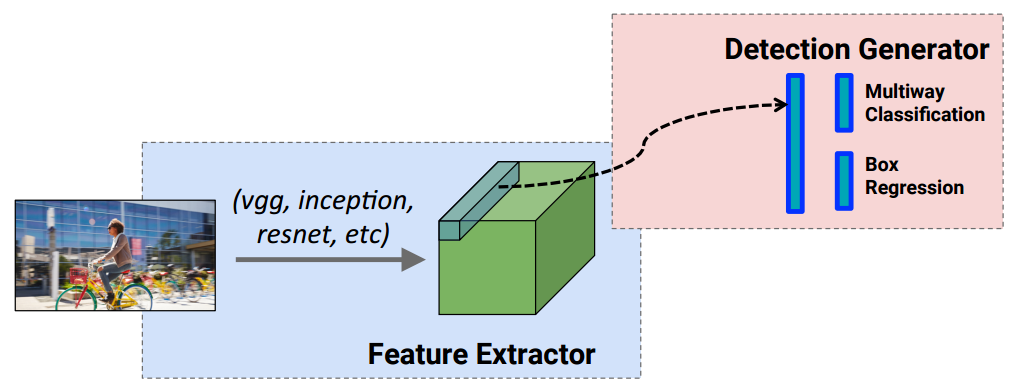
\includegraphics[width=10cm]{images/SSD_schematic}
	\caption{Schema of the SSD architecture.}
	\label{fig:perception_ssd}
\end{figure}


This network provides an accurate and efficient object detection, returning for each processed image:
\begin{itemize}
	\item \emph{Classes:} the detected classes (person, cell phone, airplane, dog \dots) inferred for each detected object.
	\item \emph{Scores:} the confidence $\in [0,1]$ the network has on each object belonging to the estimated class.
	\item \emph{Boxes:} the coordinates of the rectangular \emph{bounding box} which wraps the detected object, expressed as the coordinates of two opposite corners of it.
\end{itemize}

Although the used SSD model is capable to detect up to 80 object classes, the proposed system only retains those detection corresponding to \emph{persons}, as it is what we are interested to follow.This whole process provides a lightweight \emph{person detection}, perfectly capable to work in real time on a regular computer.

In addition, our implementation is capable to handle different network models and architectures on a \emph{plug and play} way, just pointing the model file (in the specific TensorFlow \texttt{.pb} format) in the configuration file of the program.


\subsection{Face detection}

Once the existing persons on the image have been detected, the next step is to search their faces, in order to know whether any of them corresponds to the target person to follow. In order to achieve it, the classical Viola and Jones face detection algorithm \cite{viola-jones} has been used, as it is a simple and fast solution, suitable for a prototype that already handles a \emph{SSD} CNN. This algorithm, which comprises \emph{Haar} features (Fig. \ref{fig:perception_haar}), is a simple algebraic method which takes advantage of the typical illumination pattern of a face (due to its physical shape) to detect promising regions of the input image to contain a face. To test a \emph{Haar} feature on a specific grayscale image, the feature is slided through it, and a simple operation is performed (black pixels subtracted to white ones). If the result is positive along all the feature, the region where it has been applied passes the test.


As the previous block detected persons inside the image, this face detection algorithm is only applied inside the instance of the detected persons, in order to speed up the system and avoid false positive detections. Each one of the detected persons is divided into \emph{regions}, which are passed through a \emph{cascade} of tests, where the non-compliant regions are immediately discarded. The accepted ones pass to a slightly more complex feature each time, and the regions which pass all the features are supposed to contain a face. This progressive region dismiss makes it an efficient algorithm, capable of run simultaneously with the rest of processes. This entire process is performed with an OpenCV\footnote{Open source image processing library.} function.

\begin{figure}[h]
	\centering
	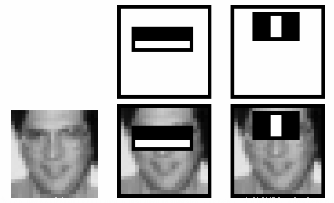
\includegraphics[width=8cm]{images/haar_on_face}
	\caption{\emph{Haar} features applied on a face.}
	\label{fig:perception_haar}
\end{figure}


\subsection{Person and face trackers}

Both previous steps detect persons and faces, but although they behave in a robust way, their outputs can suffer spurious false negative or false positive detections, due to lighting or occlusions. As they can interfere with the desired following capability, the third step palliates their effect implementing time-spatial \emph{trackers}, which filter the detection outputs (\emph{candidate detections}). The tracker associates to each person/face its coordinates inside the image, and takes into account the number of successive frames on which it has been detected. If it surpasses a \emph{patience} threshold, it is considered a reliable (\emph{tracked}) detection. Otherwise, it is taken as a spurious output and ignored. In addition, each \emph{tracked detection} is remembered for some frames even without new updates of its current position. This way, a partial occlusion of a person does not cause the her elimination, until she has not been seen for a while.
% The same happens with void detections which generally happen on a punctual way on a frame.

This tracking step can be observed in Fig. \ref{fig:perception_tracker}, in a generic \emph{instance} case (which comprises the same behavioral for person and face tracking). In addition, it is not necessary to detect the person/face every time, as the tracker is capable to infer that a new detection near the last position of a person corresponds to its new location, without needing to see again her face to check whether she is the same person.

\begin{figure}[h]
%	\centering
	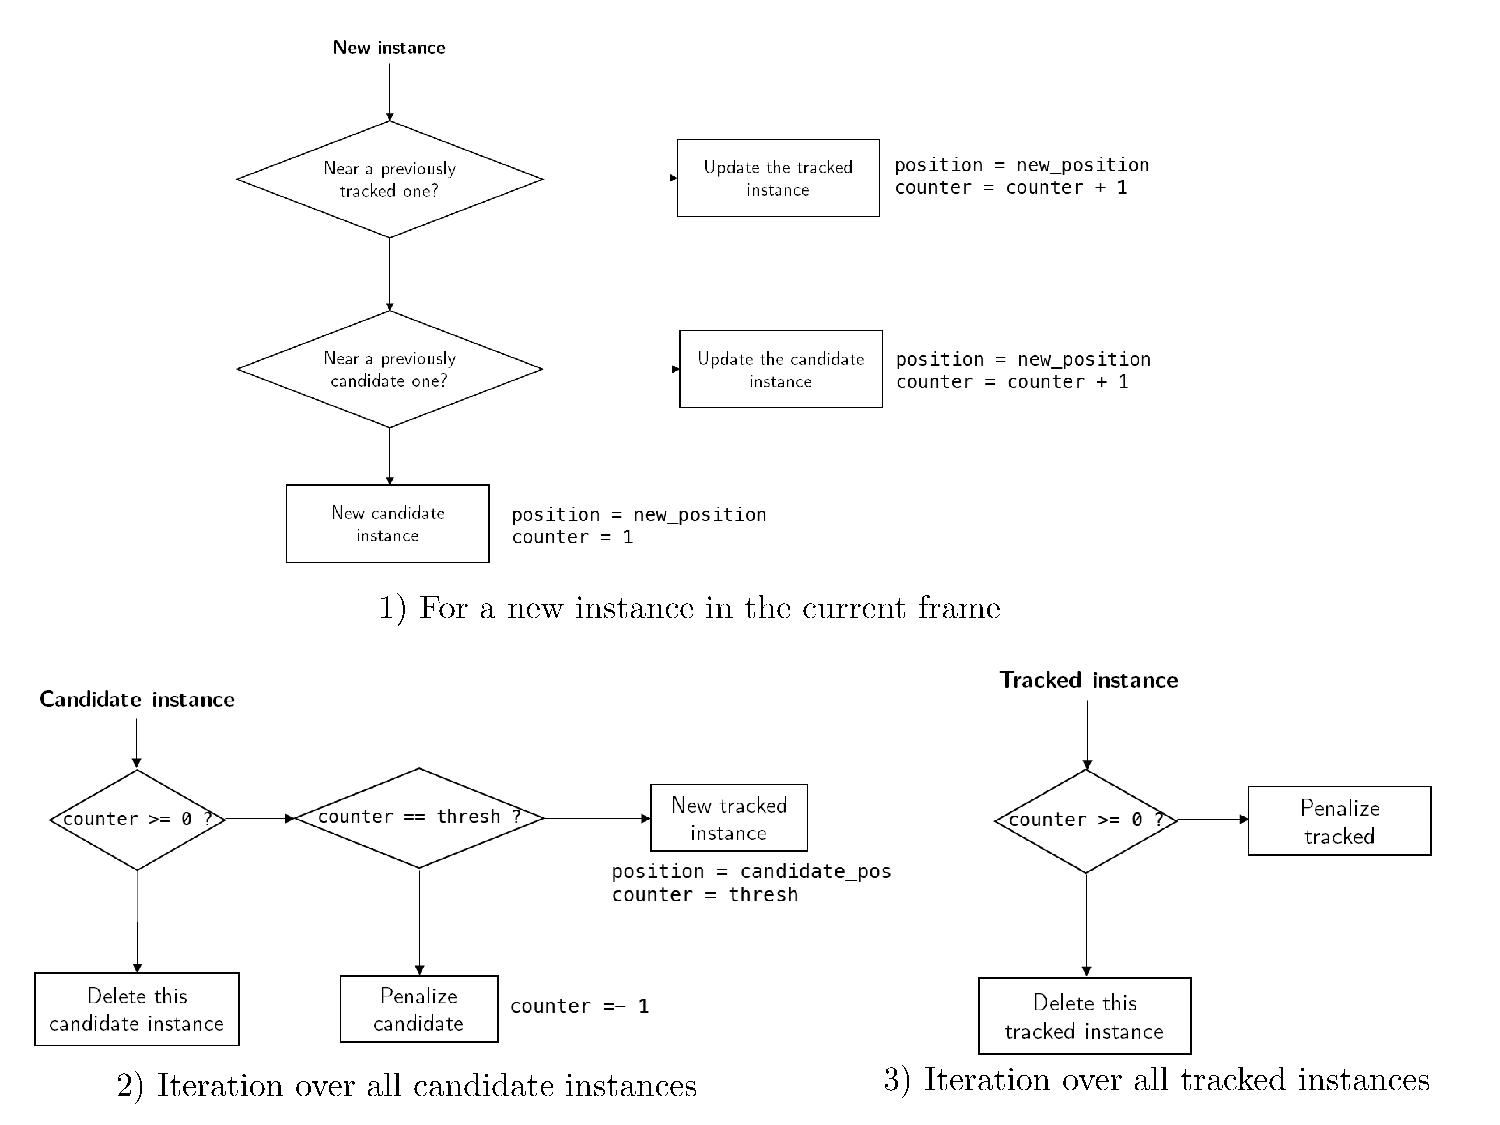
\includegraphics[width=16cm]{images/flowcharts}
	\caption{Tracking process for a instance (person/face).}
	\label{fig:perception_tracker}
\end{figure}


\subsection{Face reidentification}

The previous trackers turn the unfiltered output of the detection subsystems into tracked and more reliable detections. Hence, they can be used to perform \emph{identification} tasks. For this purpose, a parallel CNN is used, the \emph{FaceNet} \cite{facenet}. This network \emph{maps} a face image, extracting some key features, into a 128-dimensional Euclidean space, where faces are represented by what is called \emph{embeddings} (feature vectors). The Euclidean $L^2$ distance (Eq. \ref{eqn:eucl_distance}) existing between two of this embeddings stands for the \emph{face similarity} between that faces. Hence, we can consider that two embeddings belong to the same face if their distance is below a threshold, which has experimentally been set to $1.1$.

\begin{equation}
d(\vec{f_1}, \vec{f_2}) = \sqrt{\sum_{i=1}^{128}(f_{1_i} - f_{2_i})^2}
\label{eqn:eucl_distance}
\end{equation}

The proposed solution makes use of this, computing on real time the embeddings of each detected (and tracked) face. Once this has been performed, it compares the similarity between these embeddings and the one corresponding to the target person. This target embedding is computed when the program starts, from a given image file of the \emph{person to be followed}.

To avoid penalties on similarity due to lighting conditions, a previous blurring and \emph{prewhitening} (on Eq. \ref{eqn:perception_normalization}, with $x$ as the color channel, $\mu$ as its mean and $\sigma$ as its standard deviation) are performed on each given face to the \emph{FaceNet}.

\begin{equation}
x' = \frac{x - \mu}{\sigma}
\label{eqn:perception_normalization}
\end{equation}

In Figure \ref{fig:perception_distance} the same face is seen in different lighting situations, and all of them yield embeddings with a distance lower than the threshold.

\begin{figure}[h]
	\centering
	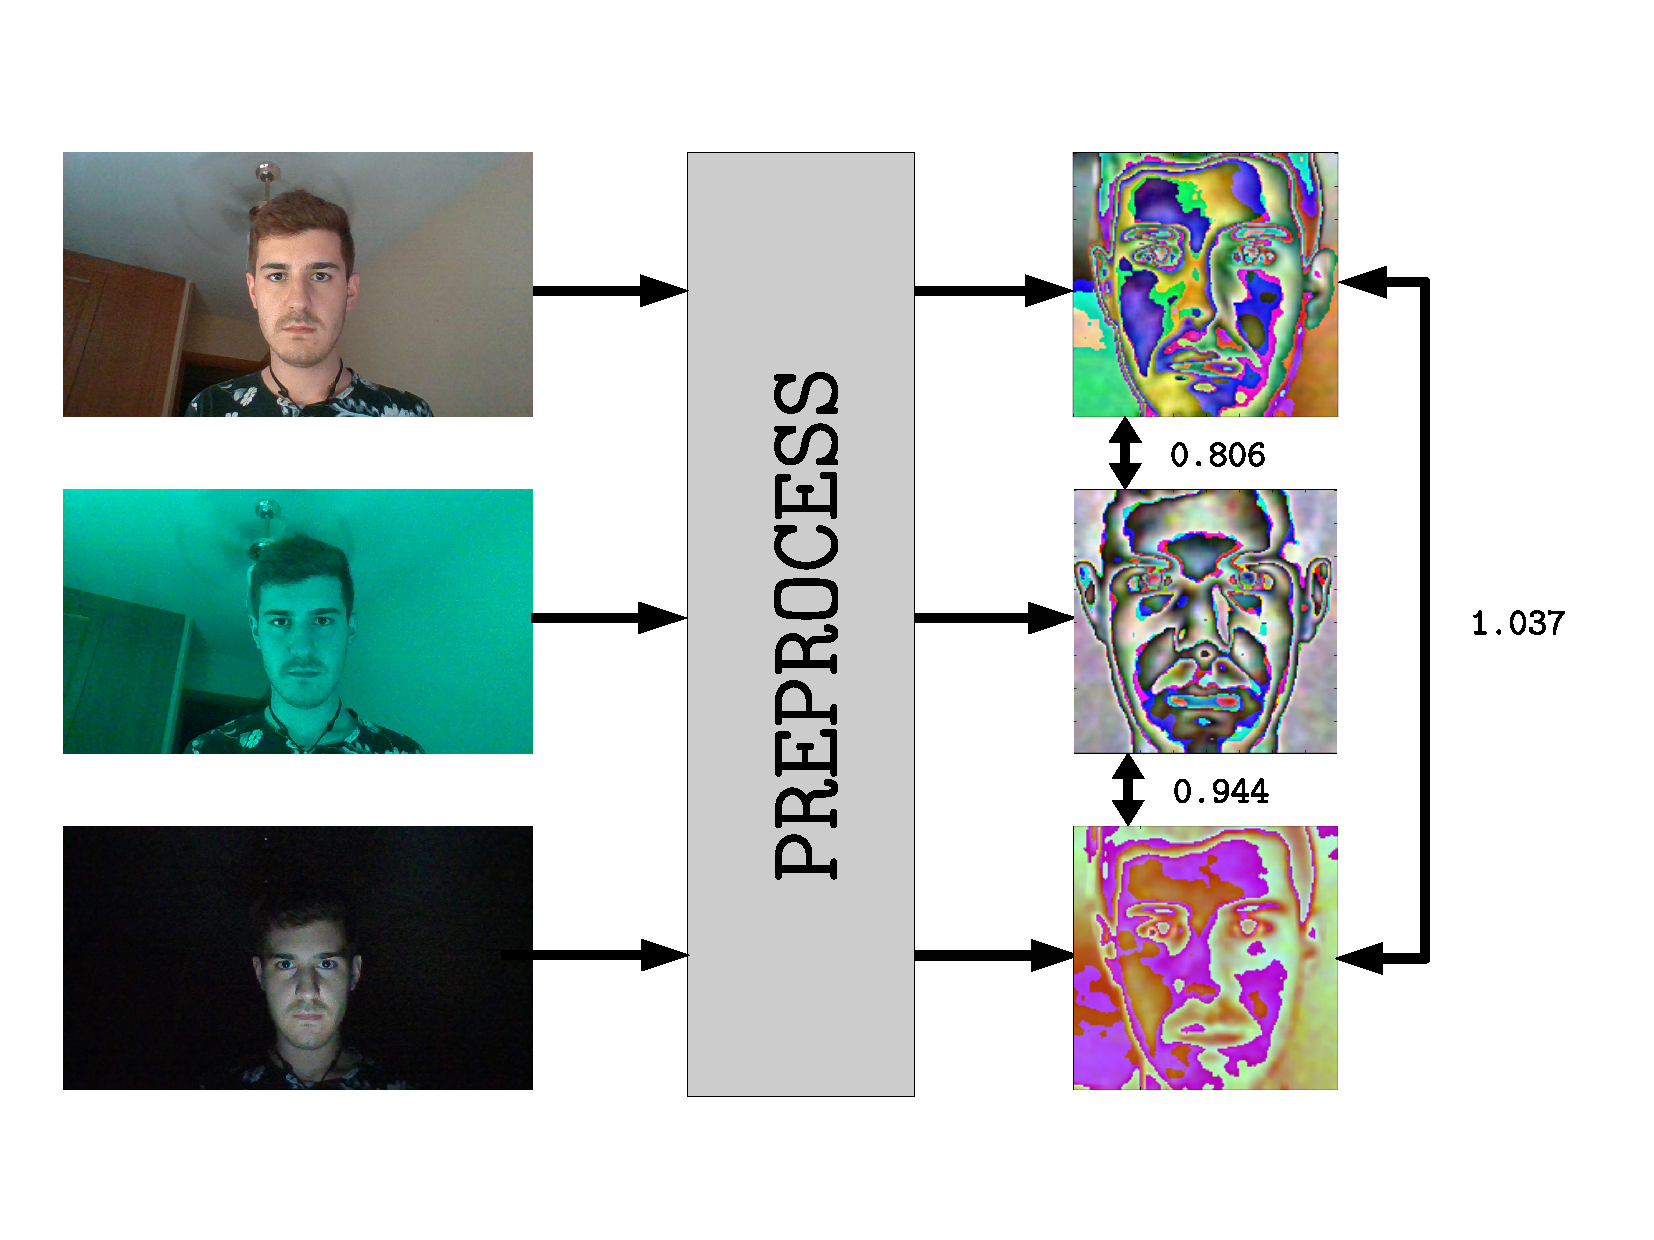
\includegraphics[width=10cm]{images/facenet_prewhiten}
	\caption{Relative distances between the same face on different lighting situations.}
        \label{fig:perception_distance}
% Color patterns on the right images are not representative, as they depend on the numeric range of the plotted image.}
\end{figure}





